% Prototype of the 13-day capture: three photographs at one height across
% \textwidth, callouts drawn by TikZ in the document font (nothing is drawn
% into the pixels). Panel height \protoH; widths follow each photo's aspect.
\newlength{\protoH}\setlength{\protoH}{1.85in}
\tikzset{
  callout/.style={font=\footnotesize, fill=white, fill opacity=0.92, text opacity=1,
                  inner sep=2pt, rounded corners=1pt, draw=none},
  calloutline/.style={-{Stealth[length=1.6mm,width=1.2mm]}, line width=0.6pt, draw=white,
                      double=black!80, double distance=0.35pt},
}
\begin{subfigure}[t]{0.219\textwidth}\centering
\begin{tikzpicture}
  \node[anchor=south west, inner sep=0] (img) {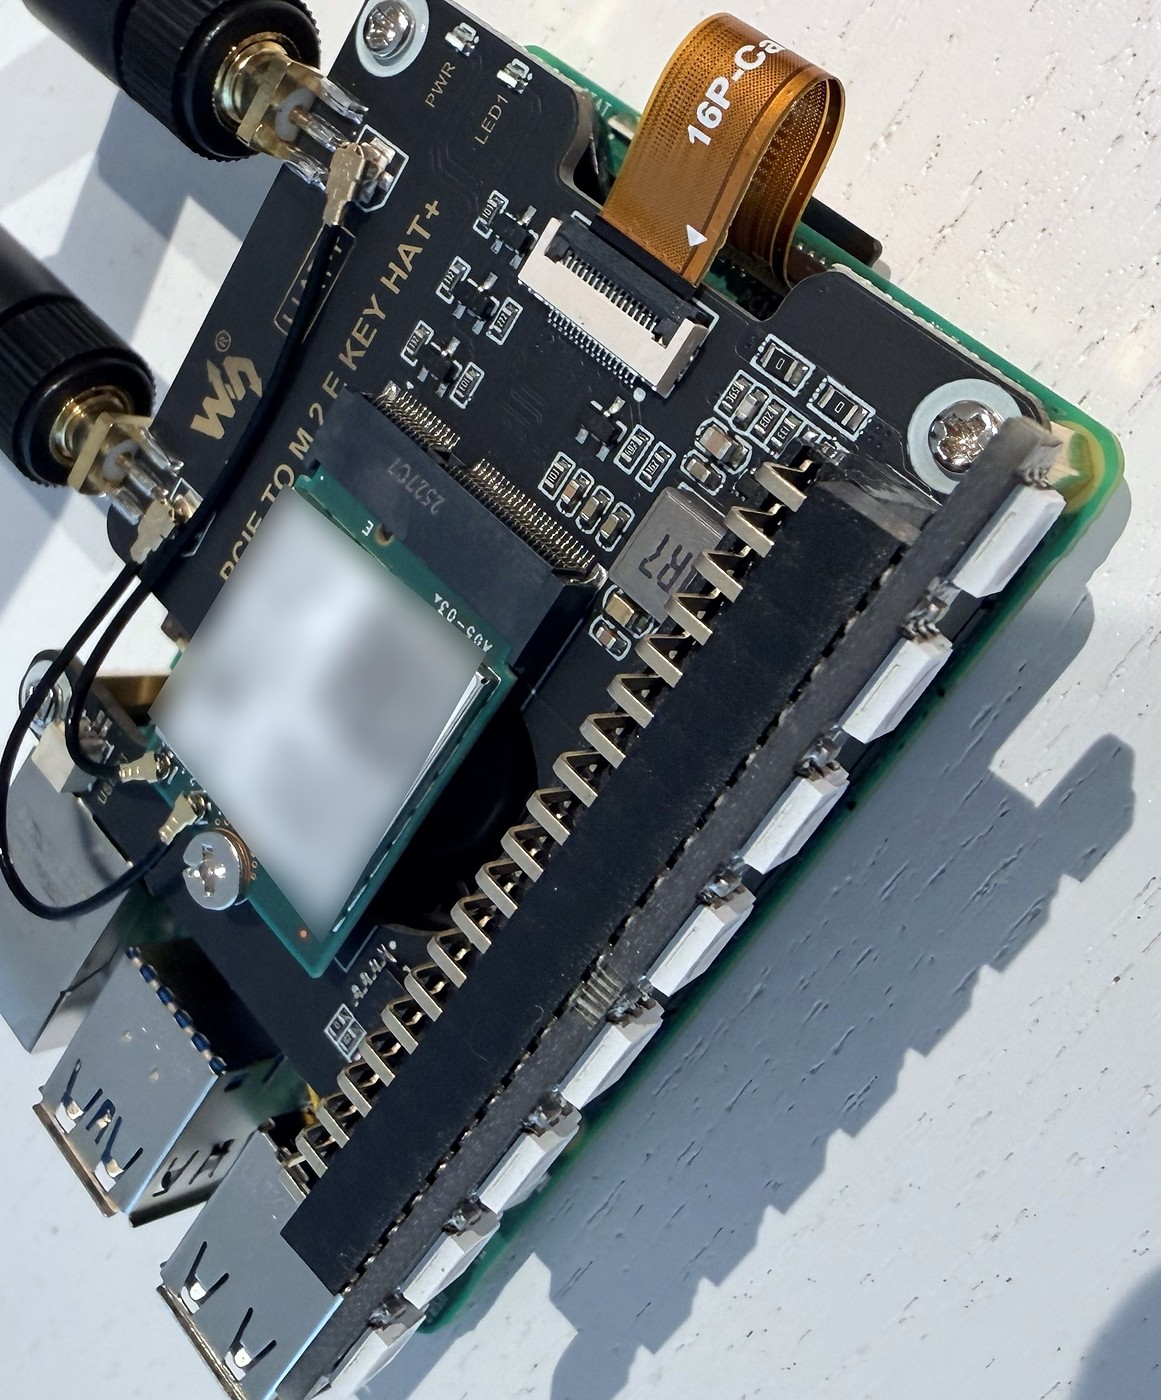
\includegraphics[height=\protoH]{figures/photo_pi_hat.jpg}};
  \begin{scope}[x={(img.south east)}, y={(img.north west)}]
    \draw[calloutline] (0.55,0.80) -- (0.27,0.57);
    \node[callout, anchor=south east, align=left] at (0.96,0.80) {Intel AX210 (M.2),\\802.11ax};
    \draw[calloutline] (0.70,0.18) -- (0.60,0.33);
    \node[callout, anchor=north east] at (0.96,0.16) {Raspberry Pi 5};
  \end{scope}
\end{tikzpicture}
\caption{}\label{fig:proto:hat}
\end{subfigure}\hfill
\begin{subfigure}[t]{0.178\textwidth}\centering
\begin{tikzpicture}
  \node[anchor=south west, inner sep=0] (img) {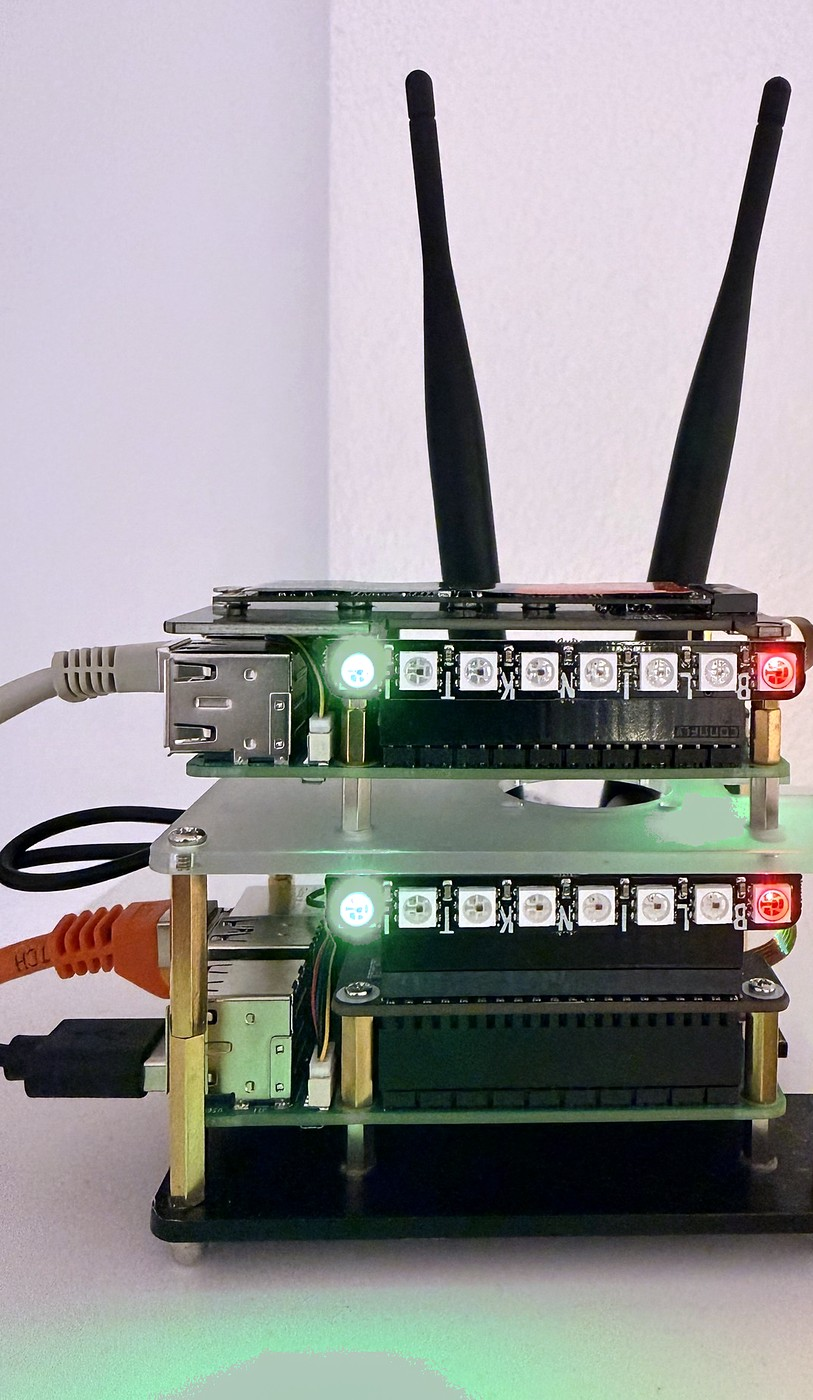
\includegraphics[height=\protoH]{figures/photo_pi_stack.jpg}};
  \begin{scope}[x={(img.south east)}, y={(img.north west)}]
    \draw[calloutline] (0.30,0.66) -- (0.42,0.58);
    \node[callout, anchor=south west] at (0.03,0.66) {storage Pi~5};
    \draw[calloutline] (0.30,0.20) -- (0.42,0.30);
    \node[callout, anchor=north west] at (0.03,0.20) {radio Pi~5};
  \end{scope}
\end{tikzpicture}
\caption{}\label{fig:proto:stack}
\end{subfigure}\hfill
\begin{subfigure}[t]{0.195\textwidth}\centering
\begin{tikzpicture}
  \node[anchor=south west, inner sep=0] (img) {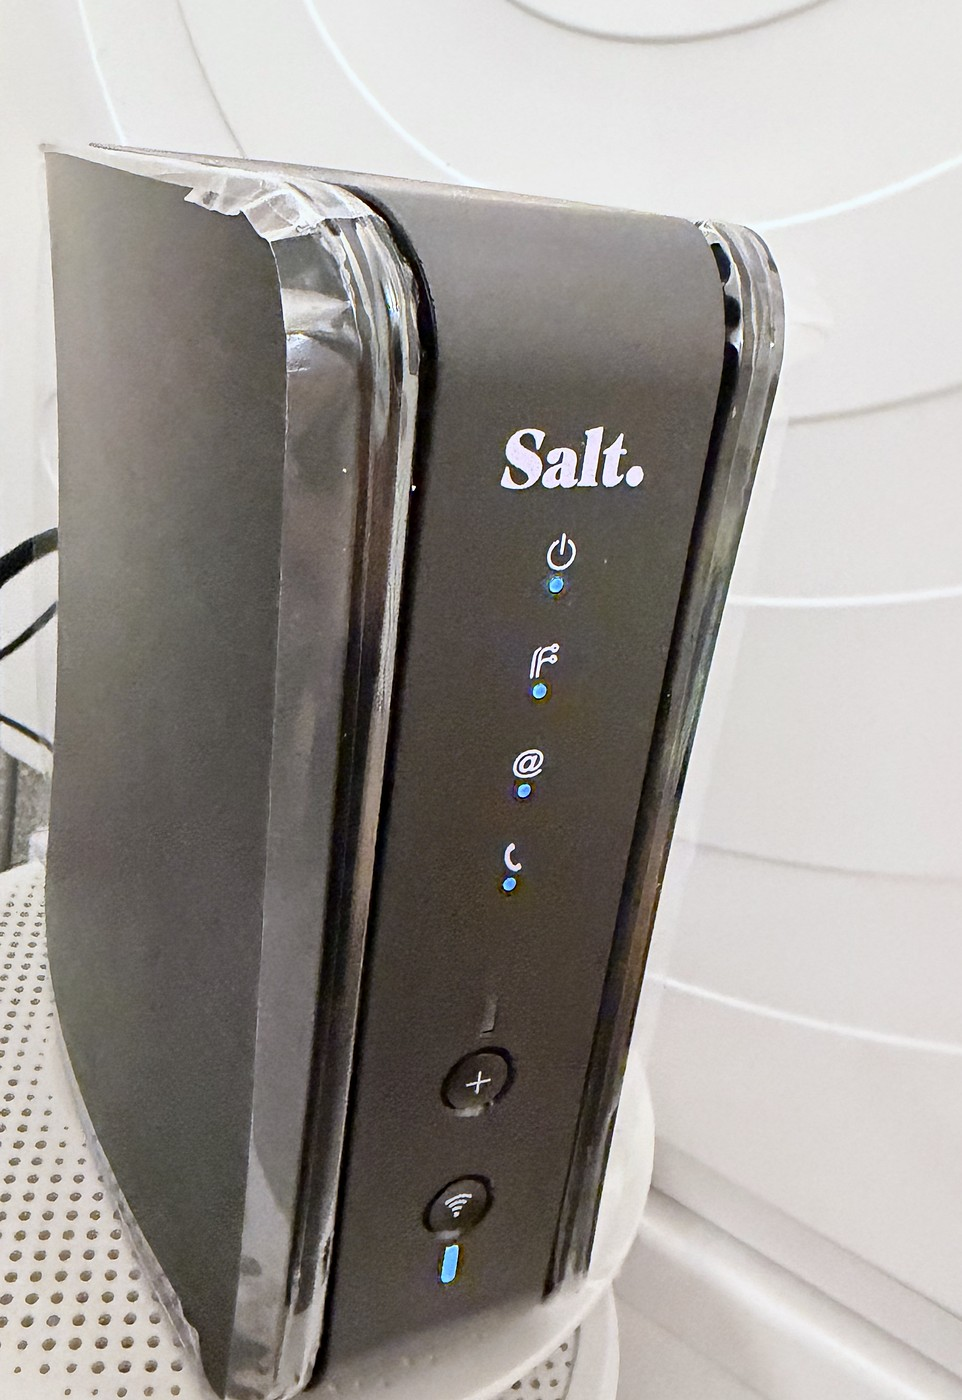
\includegraphics[height=\protoH]{figures/photo_router.jpg}};
  \begin{scope}[x={(img.south east)}, y={(img.north west)}]
    \draw[calloutline] (0.36,0.88) -- (0.55,0.72);
    \node[callout, anchor=south west] at (0.03,0.88) {gateway, 802.11be};
  \end{scope}
\end{tikzpicture}
\caption{}\label{fig:proto:router}
\end{subfigure}\hfill
\begin{subfigure}[t]{0.357\textwidth}\centering
\begin{tikzpicture}
  \node[anchor=south west, inner sep=0] (img) {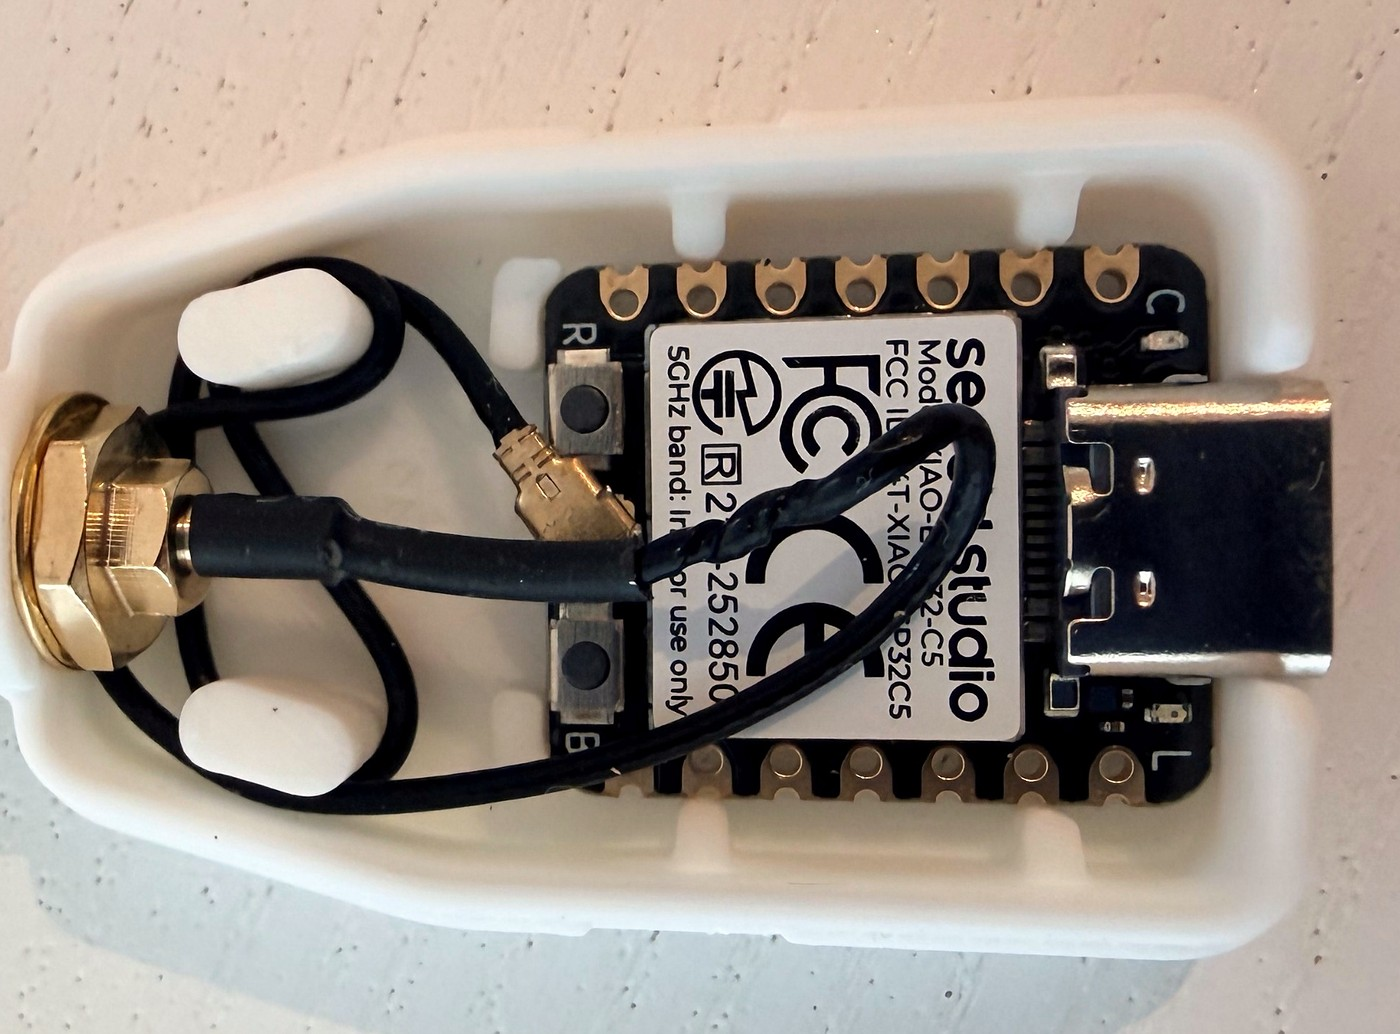
\includegraphics[height=\protoH]{figures/photo_c5.jpg}};
  \begin{scope}[x={(img.south east)}, y={(img.north west)}]
    \node[callout, anchor=north west, align=left] (c5) at (0.04,0.97) {ESP32-C5, dual-band\\802.11ax (2.4/5\,GHz)};
    \draw[calloutline] (c5.south east) -- (0.66,0.72);
    \draw[calloutline] (0.18,0.14) -- (0.10,0.40);
    \node[callout, anchor=north west] at (0.04,0.14) {external antenna};
  \end{scope}
\end{tikzpicture}
\caption{}\label{fig:proto:c5}
\end{subfigure}
